% Reporte formal del Proyecto Parcial 2 de Gestión DevOps.
% Compilación desde el directorio docs:
%   tectonic reporte.tex
% Los datos entre <> deben completarse después de las fases 9--14.

\documentclass[12pt,a4paper]{article}

\usepackage[utf8]{inputenc}
\usepackage[T1]{fontenc}
\usepackage[spanish]{babel}
\usepackage{lmodern}
\usepackage{microtype}
\usepackage[a4paper,top=2.5cm,bottom=2.5cm,left=3cm,right=2.5cm]{geometry}
\usepackage{graphicx}
\usepackage{booktabs}
\usepackage{array}
\usepackage{longtable}
\usepackage{tabularx}
\usepackage{enumitem}
\usepackage{float}
\usepackage{caption}
\usepackage{xcolor}
\usepackage{fancyhdr}
\usepackage{titlesec}
\usepackage{hyperref}
\usepackage{listings}
\usepackage{tikz}
\usetikzlibrary{arrows.meta,positioning,fit,shapes.geometric}

\definecolor{uteqBlue}{HTML}{123B63}
\definecolor{softBlue}{HTML}{EAF2F8}
\definecolor{softGray}{HTML}{F3F4F6}
\definecolor{codeGray}{HTML}{263238}
\definecolor{pendingOrange}{HTML}{B45309}

\hypersetup{
  colorlinks=true,
  linkcolor=uteqBlue,
  urlcolor=uteqBlue,
  citecolor=uteqBlue,
  pdftitle={Gestión de Procesos: CI/CD, pruebas automatizadas y observabilidad},
  pdfauthor={Sergio Abdiel Gonzalez Bravo},
  pdfsubject={Proyecto Parcial 2 de Gestión DevOps},
  pdfkeywords={DevOps, CI/CD, AWS EC2, Docker, OpenTelemetry, OpenObserve, Jest, Playwright}
}

\setlength{\parindent}{0.5cm}
\setlength{\parskip}{0.35em}
\setlist{itemsep=0.25em,topsep=0.35em}
\captionsetup{font=small,labelfont=bf}
\renewcommand{\arraystretch}{1.18}

\titleformat{\section}{\normalfont\Large\bfseries\color{uteqBlue}}{\thesection}{0.7em}{}
\titleformat{\subsection}{\normalfont\large\bfseries\color{uteqBlue}}{\thesubsection}{0.6em}{}
\titleformat{\subsubsection}{\normalfont\normalsize\bfseries\color{uteqBlue}}{\thesubsubsection}{0.5em}{}

\pagestyle{fancy}
\fancyhf{}
\fancyhead[L]{\small Gestión DevOps --- Proyecto Parcial 2}
\fancyhead[R]{\small Sergio Abdiel Gonzalez Bravo}
\fancyfoot[C]{\thepage}
\renewcommand{\headrulewidth}{0.4pt}

\lstdefinestyle{code}{
  backgroundcolor=\color{codeGray},
  basicstyle=\ttfamily\footnotesize,
  keywordstyle=\color{cyan!70!white},
  commentstyle=\color{green!60!white},
  stringstyle=\color{orange!85!white},
  numbers=left,
  numberstyle=\tiny\color{gray},
  frame=single,
  rulecolor=\color{gray!45},
  breaklines=true,
  breakatwhitespace=false,
  showstringspaces=false,
  columns=fullflexible,
  keepspaces=true,
  tabsize=2
}

\newcommand{\repoURL}{https://github.com/Chekito2720/DEVOPS}
\newcommand{\ecURL}{http://[IP\_EC2]}
\newcommand{\healthURL}{http://[IP\_EC2]/api/health}
\newcommand{\observeURL}{http://[IP\_EC2]:5080}
\newcommand{\adminCredential}{admin@demo.com}
\newcommand{\adminPassword}{[ADMIN\_PASSWORD de la EC2]}
\newcommand{\observeCredential}{[OPENOBSERVE\_USER / token de ingesta]}
\newcommand{\observePassword}{[OPENOBSERVE\_PASSWORD / token de ingesta]}

\newcommand{\pendingfigure}[2]{%
  \begin{figure}[H]
    \centering
    \fbox{%
      \begin{minipage}{0.88\linewidth}
        \centering
        \vspace{1.2cm}
        {\color{pendingOrange}\textbf{Evidencia pendiente de EC2/GitHub}}\\[0.5em]
        #2
        \vspace{1.2cm}
      \end{minipage}%
    }
    \caption{#1}
  \end{figure}
}

\begin{document}

% ============================ PORTADA ============================
\begin{titlepage}
  \centering
  \vspace*{0.5cm}
  {\color{uteqBlue}\rule{\textwidth}{1.2pt}}\\[0.8cm]
  {\Large\bfseries\color{uteqBlue} UNIVERSIDAD TECNOLÓGICA DE ECATEPEC}\\[0.25cm]
  {\large\color{uteqBlue}División de Estudios Superiores}\\[0.25cm]
  {\large\color{uteqBlue}Ingeniería en Sistemas Computacionales}\\[1.2cm]
  {\color{uteqBlue}\rule{\textwidth}{0.5pt}}\\[1.5cm]

  {\Huge\bfseries Gestión de Procesos\par}
  \vspace{0.4cm}
  {\Large Arquitectura de Entrega Continua, Pruebas Automatizadas y Observabilidad\par}
  \vspace{1.2cm}
  {\large Proyecto Parcial 2 --- Gestión DevOps\par}
  \vspace{2.2cm}

  \begin{minipage}{0.78\textwidth}
    \color{uteqBlue}\rule{\linewidth}{0.7pt}\\[0.6cm]
    \renewcommand{\arraystretch}{1.55}
    \begin{tabularx}{\linewidth}{>{\bfseries}l X}
      Autor & Sergio Abdiel Gonzalez Bravo \\
      Grupo & IDGS15 \\
      Materia & Gestión DevOps \\
      Docente & [Nombre del docente por confirmar] \\
      Repositorio & \url{\repoURL} \\
      Fecha & 22 de noviembre de 2026 \\
    \end{tabularx}
  \end{minipage}

  \vfill
  {\color{uteqBlue}\rule{\textwidth}{0.5pt}}\\[0.35cm]
  {\small Este documento se preparó con resultados reproducibles del entorno local. Las evidencias de EC2, GitHub Actions, OpenObserve y las demostraciones A/B se incorporan después de completar las fases 9--14.}
\end{titlepage}

\clearpage
\pagenumbering{roman}
\tableofcontents
\clearpage
\listoffigures
\clearpage
\listoftables
\clearpage
\pagenumbering{arabic}

% ============================ INTRODUCCIÓN ============================
\section{Introducción}

La entrega continua de software moderno exige algo más que publicar una aplicación: cada cambio debe poder verificarse de manera automatizada, construir un artefacto reproducible, desplegarse sin intervención manual indebida y dejar evidencia técnica de su operación. Este proyecto aplica ese ciclo a un sistema web de gestión compuesto por autenticación, usuarios, productos, categorías y pedidos. La solución conserva el protocolo TCP legado del ejercicio anterior, pero incorpora una API REST con contrato uniforme, autenticación JWT, una interfaz web adaptable, persistencia SQLite migrable y telemetría mediante OpenTelemetry.

El problema central no consiste únicamente en programar los endpoints. Un cambio que compila localmente puede introducir una regresión, agotar el espacio de una instancia, publicar una imagen con dependencias incorrectas o despliegarse aunque las pruebas hayan fallado. Por ello se construyó un pipeline de cinco etapas en GitHub Actions: las pruebas unitarias y de integración y las pruebas end-to-end se ejecutan en paralelo; la construcción y publicación de la imagen dependen del éxito de ambas; el despliegue por SSH depende de la imagen; y un job de reporte se ejecuta siempre para conservar el resultado de cada etapa, incluso cuando una etapa falla o es omitida.

La observabilidad complementa el control del ciclo de vida. La aplicación instrumentada produce logs estructurados, un contador de solicitudes, un histograma de latencia y trazas que incluyen operaciones de base de datos. En la instancia EC2, un OpenTelemetry Collector agrega la telemetría de la aplicación con métricas del sistema anfitrión mediante el receptor \texttt{host\_metrics}. OpenObserve almacena y permite consultar logs, métricas y trazas, así como los eventos del pipeline en el stream separado \texttt{ci\_pipeline}.

El objetivo general es demostrar un flujo DevOps verificable de extremo a extremo: código versionado, calidad comprobada, imagen contenizada, despliegue automatizado, salud verificada y telemetría centralizada. El alcance se documenta con honestidad: una EC2 es una máquina virtual y normalmente no expone sensores térmicos reales al sistema operativo; por consiguiente, no se fabrica una gráfica de temperatura y se explica explícitamente dicha limitación.

\section{Objetivos y alcance}

\subsection{Objetivo general}
Implementar y validar una plataforma web con entrega continua, despliegue automatizado en AWS EC2 y observabilidad centralizada en OpenObserve, conservando las funcionalidades legadas y incorporando pruebas automáticas que protejan el despliegue.

\subsection{Objetivos específicos}
\begin{enumerate}
  \item Implementar autenticación JWT, administration de usuarios y CRUD de productos con validaciones de entrada.
  \item Mantener un contrato JSON REST consistente con metadatos de respuesta y conservar el contrato TCP 6061.
  \item Proteger la base SQLite y migrar de forma verificable el esquema de la práctica anterior.
  \item Medir la cobertura con Jest y Supertest, y validar la interfaz y la API con Playwright.
  \item Construir una imagen multi-stage ligera y no root sobre Node.js 22.
  \item Condicionar el despliegue a la aprobación completa de las pruebas.
  \item Enviar logs, métricas, trazas y eventos CI/CD a OpenObserve.
  \item Documentar la operación, los secretos y la preparación de EC2 sin exponer credenciales en el repositorio.
\end{enumerate}

\subsection{Alcance}
El sistema mínimo del parcial incluye login y CRUD de usuarios y productos en frontend y backend. La solución también conserva categorías, pedidos, respaldos y el puerto TCP 6061. La trazabilidad de infraestructura corresponde a CPU, RAM, disco, red y carga. La temperatura real de hardware queda fuera del alcance por la naturaleza virtualizada de EC2.

% ============================ ARQUITECTURA ============================
\section{Arquitectura de la solución}

La arquitectura separa control del ciclo de entrega, ejecución de la aplicación, recolección de telemetría y almacenamiento. GitHub Actions decide si una versión puede desplegarse; Docker Hub conserva las imágenes inmutables por hash del commit y la etiqueta \texttt{latest}; EC2 ejecuta la pila con Docker Compose; el Collector normaliza y reenvía señales; OpenObserve ofrece la consulta centralizada.

\begin{figure}[H]
  \centering
  \resizebox{\textwidth}{!}{%
  \begin{tikzpicture}[
    node distance=9mm and 13mm,
    every node/.style={font=\small,align=center},
    box/.style={draw=uteqBlue,rounded corners,fill=softBlue,minimum width=37mm,minimum height=13mm},
    cloud/.style={draw=uteqBlue,fill=softGray,rounded corners,minimum width=37mm,minimum height=13mm},
    arrow/.style={-{Latex[length=2.2mm]},thick,draw=uteqBlue}
  ]
    \node[box] (dev) {Desarrollador\\\texttt{git push main}};
    \node[box,right=of dev] (gha) {\textbf{GitHub Actions}\\\texttt{test} y \texttt{e2e}\\\texttt{build} $\rightarrow$ \texttt{deploy}};
    \node[cloud,right=of gha] (hub) {Docker Hub\\\texttt{latest} + \texttt{sha}};
    \node[box,right=of hub] (ec2) {\textbf{AWS EC2 / Ubuntu}\\API + Collector};
    \node[box,below=of ec2] (oo) {OpenObserve\\logs, métricas, trazas};
    \node[box,left=of ec2] (api) {API Node.js\\\texttt{api-cicd}:80\\\texttt{TCP}:6061};
    \node[box,left=of api] (otel) {OTel Collector\\\texttt{host\_metrics}};
    \node[box,below=of api] (db) {Volumen \texttt{api\_data}\\SQLite};

    \draw[arrow] (dev) -- (gha);
    \draw[arrow] (gha) -- node[above,font=\scriptsize]{imagen} (hub);
    \draw[arrow] (hub) -- (ec2);
    \draw[arrow] (ec2) -- (api);
    \draw[arrow] (api) -- (otel);
    \draw[arrow] (otel) -- (oo);
    \draw[arrow] (api) -- (db);
    \draw[arrow] (gha.south) |- node[pos=0.72,left,font=\scriptsize]{eventos CI/CD} (oo.south);
  \end{tikzpicture}%
  }
  \caption{Arquitectura de CI/CD y observabilidad. Las flechas representan publicación de imágenes, despliegue, telemetría OTLP y registro de eventos del pipeline.}
  \label{fig:arquitectura}
\end{figure}

\subsection{Componentes y responsabilidades}

\begin{table}[H]
  \centering
  \caption{Componentes del sistema y responsabilidad principal.}
  \begin{tabularx}{\textwidth}{>{\bfseries}p{3.2cm} X}
    \toprule
    Componente & Responsabilidad \\
    \midrule
    GitHub Actions & Ejecutar pruebas paralelas, publicar la imagen, desplegar bajo condiciones y registrar resultados. \\
    GitHub Secrets & Entregar credenciales sin escribirlas en código ni en los logs del repositorio. \\
    Docker Hub & Almacenar la imagen publicada con etiqueta \texttt{latest} y etiqueta igual al SHA del commit. \\
    API Node.js & Servir frontend y API REST, autenticar, validar, persistir y emitir telemetría. \\
    SQLite & Conservar usuarios, productos, categorías y pedidos; mantener el volumen entre despliegues. \\
    OTel Collector & Recibir OTLP, recolectar métricas del host y exportar a OpenObserve. \\
    OpenObserve & Persistir y consultar logs, métricas, trazas y el stream \texttt{ci\_pipeline}. \\
    \bottomrule
  \end{tabularx}
\end{table}

% ============================ DESARROLLO ============================
\section{Desarrollo del sistema}

\subsection{Backend REST y contrato de respuestas}

El backend utiliza Express 5 y \texttt{better-sqlite3}. Todas las respuestas JSON de la API ---incluidos errores de validación, autenticación y operación interna--- comparten la siguiente estructura:

\begin{lstlisting}[style=code]
{
  "statusCode": 200,
  "responseTime": 1.43,
  "request": "GET",
  "path": "/api/health",
  "timestamp": "2026-11-22T04:56:17.083Z",
  "data": { "status": "ok" }
}
\end{lstlisting}

La exclusividad entre \texttt{data} y \texttt{error} se verifica automáticamente en la suite. El campo \texttt{responseTime} expresa la latencia en milisegundos; \texttt{path} excluye el query string; y \texttt{timestamp} utiliza ISO 8601 en UTC. Esta uniformidad facilita el consumo por el frontend, los clientes de API y las herramientas de pruebas.

\begin{table}[H]
  \centering
  \caption{Endpoints REST implementados y control de acceso.}
  \small
  \begin{tabularx}{\textwidth}{l l >{\raggedright\arraybackslash}X}
    \toprule
    Método & Ruta & Acceso y propósito \\
    \midrule
    GET & \texttt{/api/health} & Público; estado del servicio. \\
    POST & \texttt{/api/auth/login} & Público; emite un JWT HS256. \\
    GET/POST/PUT/DELETE & \texttt{/api/users[/:id]} & Administrador; administration de usuarios. \\
    GET/POST/PUT/DELETE & \texttt{/api/productos[/:id]} & Usuario autenticado; inventario con \texttt{stock}. \\
    GET/POST/DELETE & \texttt{/api/categorias[/:id]} & Funcionalidad legacy conservada. \\
    GET/POST & \texttt{/api/pedidos} & Funcionalidad legacy conservada. \\
    GET & \texttt{/api/db/backup} & Administrador; respaldo SQLite. \\
    DELETE & \texttt{/api/db/clear} & Administrador; limpieza transaccional de datos operativos. \\
    \bottomrule
  \end{tabularx}
\end{table}

Las validaciones rechazan, entre otros casos, identificadores no numéricos, nombres vacíos, correos con tipo o formato incorrecto, contraseñas menores a seis caracteres, roles no permitidos, precios negativos o no finitos, stock no entero, cantidades de pedido inválidas y referencias de categoría inexistentes. Los errores de negocio se traducen a 400, 401, 403, 404 o 409 según corresponda; los fallos internos de SQLite se reportan como 500 sin exponer mensajes de implementación al cliente.

\subsection{Autenticación, autorización y revocación}

El login busca el usuario por correo normalizado y verifica la contraseña con \texttt{bcryptjs}. El JWT se firma explícitamente con el algoritmo HS256 y expira, por omisión, después de dos horas. En producción, \texttt{JWT\_SECRET} es obligatorio y debe tener al menos 32 caracteres; \texttt{ADMIN\_PASSWORD} también es obligatorio y tiene una longitud mínima.

Cada petición autenticada consulta again al usuario vigente. Además, la tabla \texttt{users} incorpora \texttt{token\_version}. Un cambio de rol o contraseña incrementa esa versión, por lo que los tokens emitidos previamente dejan de ser válidos. Si el usuario se elimina, la consulta deja de encontrarlo y su token se invalida. Esta decisión evita que un token conserve privilegios que ya fueron revocados en la base de datos.

Las operaciones de usuarios, respaldos y limpieza exigen rol \texttt{admin}. Un administrador no puede eliminarse a sí mismo ni quitarse sus propios permisos. Estas restricciones reduce la probabilidad de una intervención administrativa destructiva o de un bloqueo accidental de la única cuenta de administración.

\subsection{Base de datos, migración y respaldo}

SQLite opera con claves foráneas activas y modo WAL. Las tablas principales son \texttt{users}, \texttt{productos}, \texttt{categorias} y \texttt{pedidos}. La migración de la base legacy agrega \texttt{stock} a productos, vuelve opcional \texttt{categoria\_id}, conserva la relación con pedidos y preserva la secuencia de identificadores incluso cuando el último registro fue eliminado.

Antes de modificar una base existente se crea un respaldo \texttt{pre-migration-[timestamp].db}. La copia se realiza mediante \texttt{VACUUM INTO}, en tanto que la migración de productos se ejecuta dentro de una transacción. La prueba automatizada crea una base anterior, elimina un producto, migra, verifica conteos y claves foráneas, comprueba la secuencia y confirma que el siguiente identificador no reutiliza el ID eliminado.

El administrador bootstrap se crea únicamente cuando la tabla de usuarios no existía originalmente. Si una persona elimina deliberadamente la última cuenta administradora, el proceso no la resucita y se niega a iniciar en producción. Esta regla evita una reinstalación insegura e implícita y obliga a una recuperación explícita.

\begin{pendingfigure}{Estructura de tablas y relationships de la base SQLite en el entorno local.}{La figura definitiva puede sustituirse por una captura del esquema o por el resultado de \texttt{.schema} en la EC2.}
\label{fig:db}
\end{pendingfigure}

\subsection{Protocolo TCP legado 6061}

El servidor TCP conserva el contrato anterior \texttt{\{statusCode, data|error\}}, sin añadir metadatos REST. Se reconoce el comando de inserción \texttt{\{insert:[objeto]\}} y el de consulta \texttt{\{get:\{...\}\}}. El servidor mantiene un buffer por conexión: si un comando llega fragmentado, espera las partes restantes; si una lectura contiene varios comandos, los procesa en orden. Cada respuesta termina con salto de línea.

\begin{figure}[H]
  \centering
  \fbox{\begin{minipage}{0.85\linewidth}\centering
    \texttt{\{get:\{"id":1\}\}}\newline
    $\downarrow$\newline
    \texttt{\{"statusCode":200,"data":\{...\}}\}
  \end{minipage}}
  \caption{Formato conservado del protocolo TCP 6061.}
  \label{fig:tcp}
\end{figure}

\subsection{Frontend}

El frontend es una aplicación de una sola página, sin framework, compuesta por HTML, CSS y JavaScript nativo. Después del login muestra las vistas de productos, categorías y pedidos; la administración de usuarios se presenta únicamente a administradores. Los formularios.executes validaciones básicas del navegador y el API conserva la validación definitiva del servidor. Los valores provenientes de la base se escapan antes de construir el HTML para reducir el riesgo de inyección de scripts en el DOM.

La interfaz es adaptable a pantallas pequeñas, incluye estados visibles para éxito y error, conserva el token únicamente en \texttt{sessionStorage} y elimina la sesión cuando el API responde 401. El token se obtiene en el login y se envía como \texttt{Authorization: Bearer [token]}.

\begin{figure}[H]
  \centering
  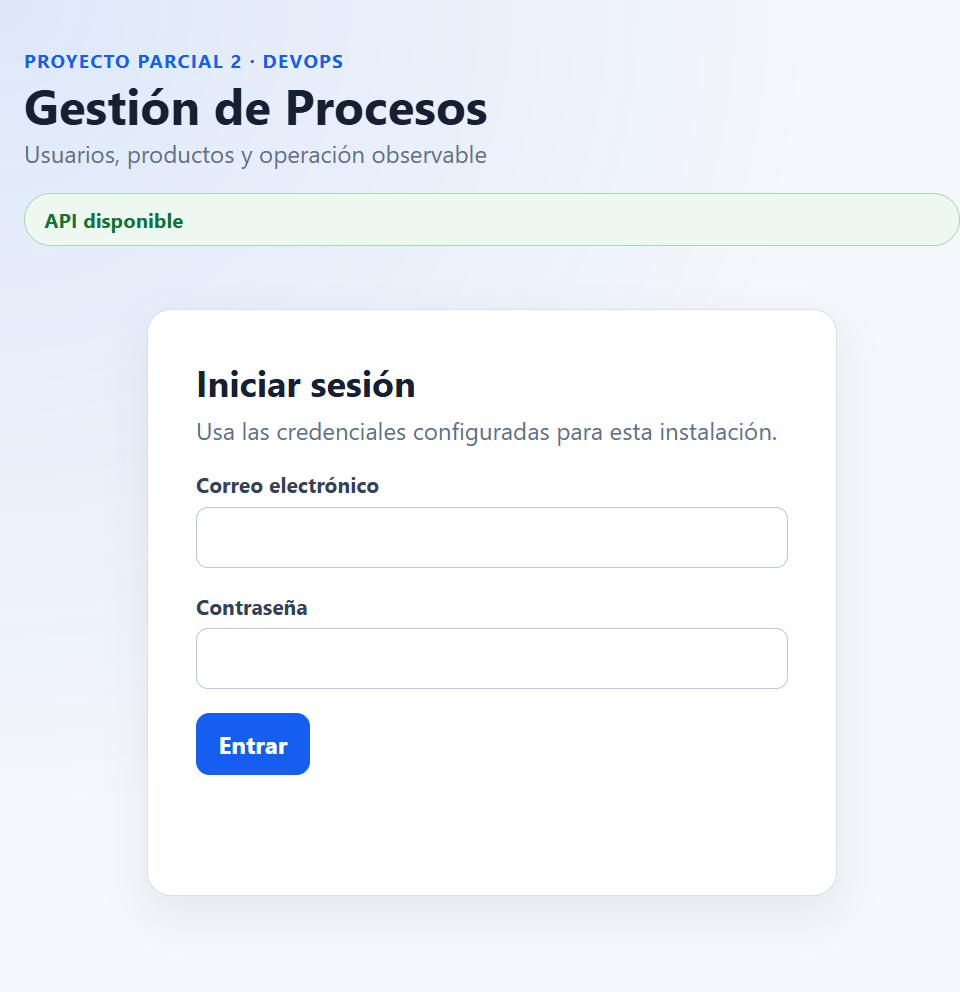
\includegraphics[width=0.72\textwidth]{figures/login-local.png}
  \caption{Pantalla de inicio de sesión de la aplicación local.}
  \label{fig:login}
\end{figure}

\begin{figure}[H]
  \centering
  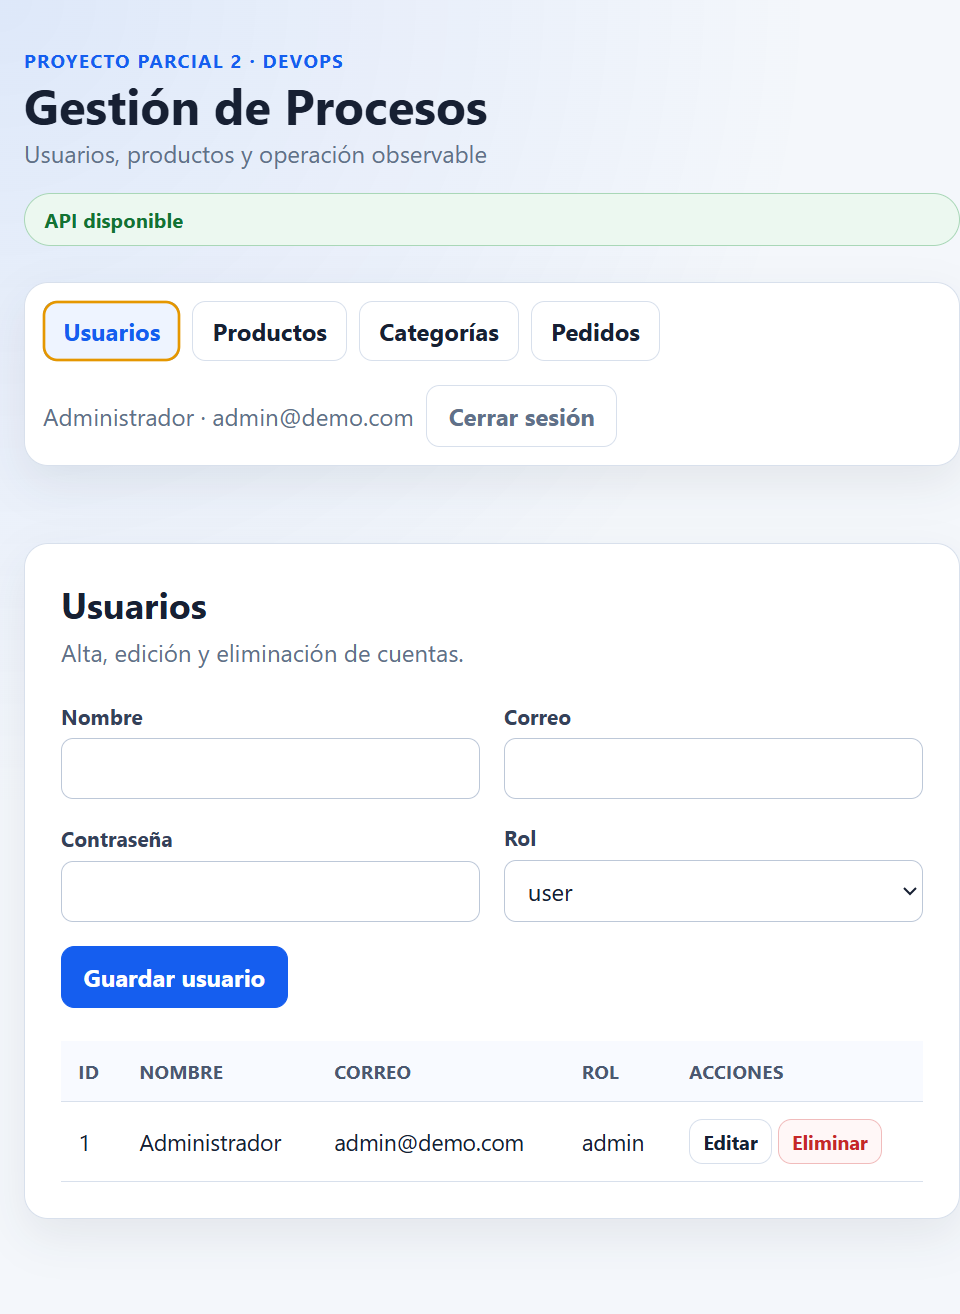
\includegraphics[width=\textwidth]{figures/usuarios-local.png}
  \caption{Administración de usuarios en la aplicación local.}
  \label{fig:usuarios}
\end{figure}

\begin{figure}[H]
  \centering
  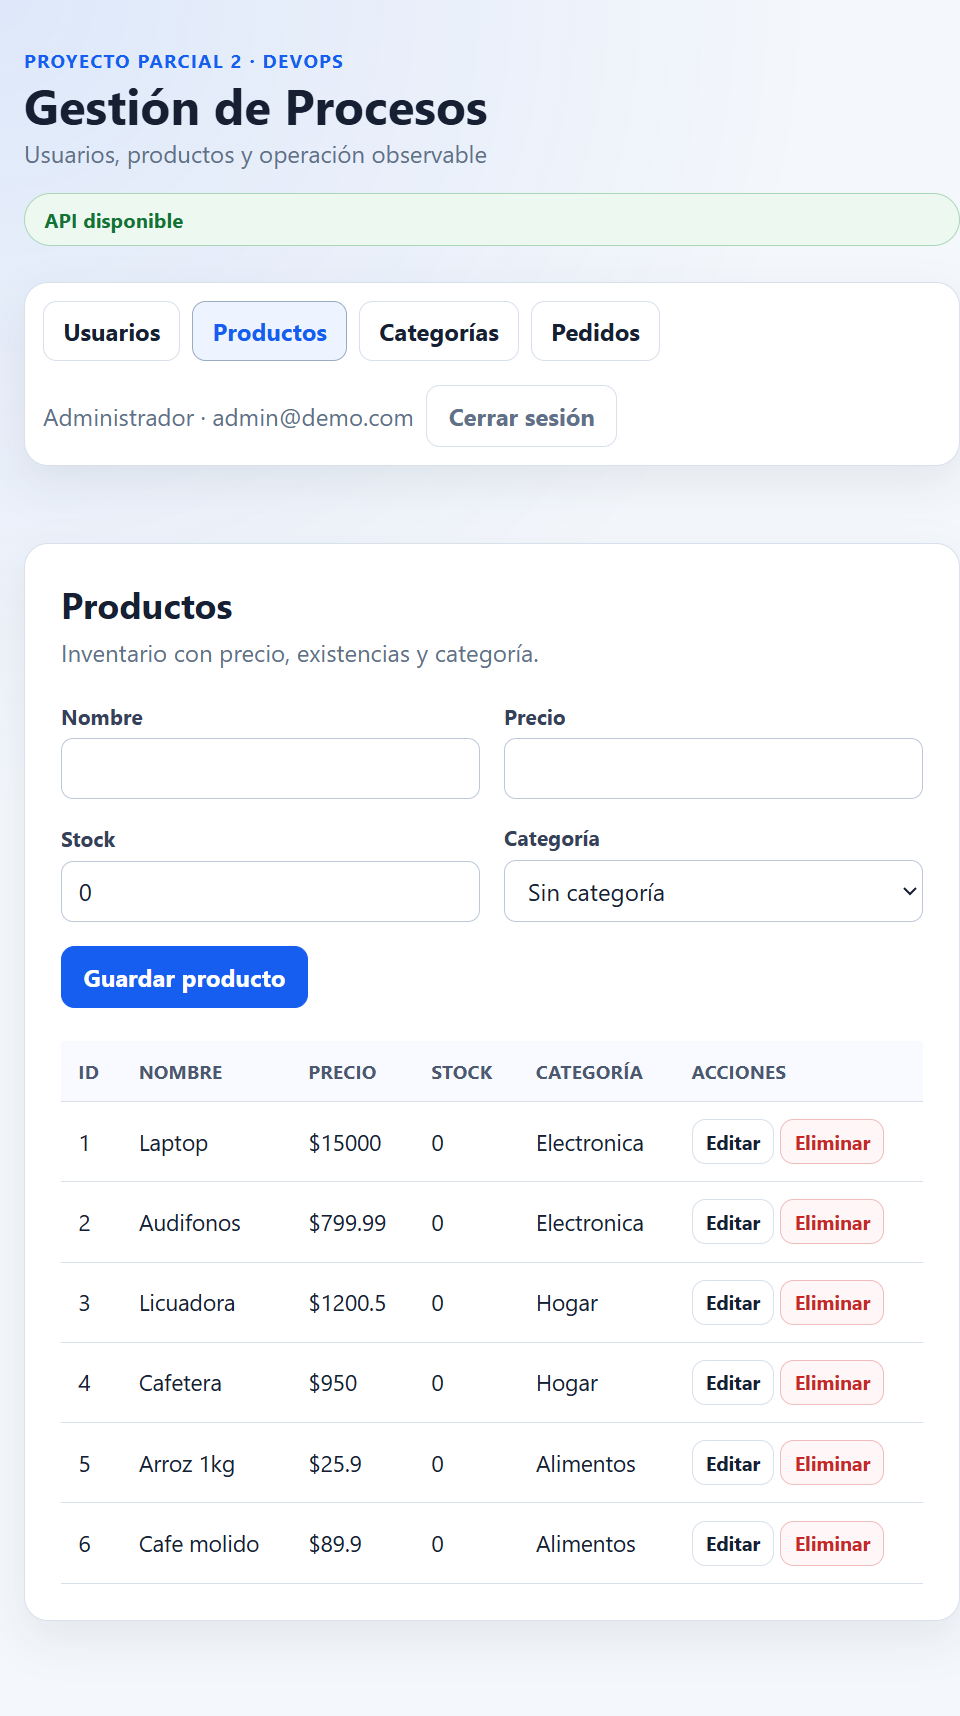
\includegraphics[width=\textwidth]{figures/productos-local.png}
  \caption{Gestión de productos en la aplicación local. Los registros proceden de la base legacy migrada, por lo que su stock inicial es cero.}
  \label{fig:productos}
\end{figure}

% ============================ PRUEBAS ============================
\section{Pruebas automatizadas}

\subsection{Jest y Supertest}

Jest ejecuta pruebas de integración sobre la aplicación Express mediante Supertest. La suite utiliza una base SQLite en memoria y restaura un conjunto reproducible antes de las pruebas; nunca modifica la base de datos real. Se configuran umbrales globales de 70\% para statements, branches, functions y lines.

\begin{table}[H]
  \centering
  \caption{Resultado de la regresión Jest ejecutada el 22 de noviembre de 2026.}
  \begin{tabular}{l r}
    \toprule
    Indicador & Resultado \\
    \midrule
    Suites & 4 aprobadas de 4 \\
    Pruebas & 93 aprobadas de 93 \\
    Statements & 76.16\% \\
    Branches & 70.09\% \\
    Functions & 89.38\% \\
    Lines & 77.95\% \\
    \bottomrule
  \end{tabular}
\end{table}

La suite comprueba el envelope exacto de respuestas correctas y fallidas, login y expiración de JWT, HS256, autorización por rol, revocación de tokens, CRUD de usuarios y productos, validaciones, errores del parser, límites de cuerpo, categorías, pedidos, respaldos, limpieza transaccional, migración legacy, secuencia SQLite, no resucitación del administrador eliminado y contrato TCP.

\begin{figure}[H]
  \centering
  \fbox{\begin{minipage}{0.84\textwidth}\centering\vspace{0.8cm}
    \textbf{Salida de cobertura Jest}\\[0.4cm]
    \texttt{93 passed, 4 suites passed}\\[0.2cm]
    \texttt{Statements 76.16\% \quad Branches 70.09\%}\\[0.2cm]
    \texttt{Functions 89.38\% \quad Lines 77.95\%}\\[0.8cm]
  \end{minipage}}
  \caption{Resumen de la última regresión Jest.}
  \label{fig:jest}
\end{figure}

\subsection{Playwright}

Playwright valida tanto la interfaz como la API. El servidor E2E se levanta con un puerto HTTP fijo, un puerto TCP efímero, SQLite en memoria y \texttt{reuseExistingServer=false}; de esta forma no se reutiliza una instancia local ni se contamina la base real. Se ejecutaron 17 pruebas en Chromium: login válido e inválido, restauración de sesión, control de visibilidad por rol, CRUD de usuarios, duplicados, CRUD de productos, validaciones de precio y stock, categorías, pedidos, health, protección de rutas y flujos REST.

\begin{table}[H]
  \centering
  \caption{Resultado de la regresión Playwright ejecutada el 22 de noviembre de 2026.}
  \begin{tabular}{l r}
    \toprule
    Indicador & Resultado \\
    \midrule
    Navegador & Chromium \\
    Pruebas E2E & 17 aprobadas de 17 \\
    Servidor & Nuevo, SQLite en memoria \\
    Puerto TCP de pruebas & Efímero \\
    Reutilización de servidor & Deshabilitada \\
    \bottomrule
  \end{tabular}
\end{table}

\begin{figure}[H]
  \centering
  \fbox{\begin{minipage}{0.84\textwidth}\centering\vspace{0.8cm}
    \textbf{Ejecución Playwright}\\[0.4cm]
    \texttt{Running 17 tests using 1 worker}\\[0.2cm]
    \texttt{17 passed (11.1s)}\\[0.8cm]
  \end{minipage}}
  \caption{Resumen de la última regresión Playwright.}
  \label{fig:playwright}
\end{figure}

% ============================ CI/CD ============================
\section{Integración continua y entrega continua}

\subsection{Organización del pipeline}

El archivo \texttt{.github/workflows/main.yml} contiene cinco jobs. \texttt{test} y \texttt{e2e} son independientes y se ejecutan en paralelo. \texttt{build-and-push} declara \texttt{needs: [test, e2e]} y una condición explícita que exige resultado \texttt{success} para ambas. \texttt{deploy} depende de la construcción correcta y abre la conexión SSH únicamente después de esa condición. \texttt{report} usa \texttt{if: always()} para registrar el resultado real de las cuatro etapas, aun cuando algunas fueron omitidas.

\begin{figure}[H]
  \centering
  \begin{tikzpicture}[
    node distance=13mm and 8mm,
    every node/.style={font=\small,align=center},
    job/.style={draw=uteqBlue,rounded corners,fill=softBlue,minimum width=28mm,minimum height=11mm},
    gate/.style={draw=pendingOrange,rounded corners,fill=orange!10,minimum width=36mm,minimum height=11mm},
    arrow/.style={-{Latex[length=2mm]},thick,draw=uteqBlue}
  ]
    \node[job] (test) {\textbf{test}\\Jest $\geq70\%$};
    \node[job,right=of test] (e2e) {\textbf{e2e}\\Playwright};
    \node[gate,right=of e2e,yshift=0cm] (build) {\textbf{build-and-push}\\ambos \texttt{success}};
    \node[job,right=of build] (deploy) {\textbf{deploy}\\SSH + health};
    \node[gate,below=of e2e] (report) {\textbf{report}\\\texttt{always()}};
    \draw[arrow] (test) -- (build);
    \draw[arrow] (e2e) -- (build);
    \draw[arrow] (build) -- (deploy);
    \draw[arrow] (test.south) |- (report);
    \draw[arrow] (e2e) -- (report);
    \draw[arrow] (build.south) |- (report);
    \draw[arrow] (deploy.south) |- (report);
  \end{tikzpicture}
  \caption{Dependencias del pipeline. La rama de despliegue es inalcanzable si una prueba falla.}
  \label{fig:pipeline}
\end{figure}

\begin{table}[H]
  \centering
  \caption{Condiciones de ejecución y seguridad de los jobs.}
  \small
  \begin{tabularx}{\textwidth}{>{\bfseries}p{3.4cm} X >{\bfseries}p{3.1cm}}
    \toprule
    Job & Condición & Resultado ante fallo \\
    \midrule
    test & Push o pull request & Falla y publica cobertura como artefacto. \\
    e2e & Push o pull request & Falla y publica reporte HTML. \\
    build-and-push & Push y \texttt{test=success} y \texttt{e2e=success} & Se omite; no publica imagen. \\
    deploy & Push y \texttt{build-and-push=success} & Se omite; no abre SSH. \\
    report & \texttt{always()} & Envía estados \texttt{success}, \texttt{failure} o \texttt{skipped}. \\
    \bottomrule
  \end{tabularx}
\end{table}

\subsection{Construcción y despliegue}

La imagen se construye con Buildx y se publica en Docker Hub con dos etiquetas: \texttt{latest} y el SHA completo del commit. La etapa de dependencias instala \texttt{better-sqlite3}; la imagen final copia únicamente dependencias de producción y código necesario, se ejecuta como usuario \texttt{node} y contiene un healthcheck contra \texttt{/api/health}. El uso de \texttt{node:22-slim} evita las limitaciones de compilación de módulos nativos observadas en variantes Alpine para las versiones empleadas.

El job de despliegue copia \texttt{docker-compose.yml} y \texttt{otel-collector-config.yaml} por SCP, exporta \texttt{IMAGE\_TAG} con el SHA, ejecuta \texttt{docker compose pull} y \texttt{docker compose up -d}, y espera hasta 60 segundos una respuesta HTTP exitosa. Si la API no se recupera, imprime logs y termina con error; el job \texttt{report} conserva ese estado.

\begin{pendingfigure}{Pipeline completo en GitHub Actions con cinco jobs en verde.}{Capturar después de la fase 12. Esta figura debe mostrar explícitamente \texttt{test}, \texttt{e2e}, \texttt{build-and-push}, \texttt{deploy} y \texttt{report}.}
\label{fig:actions}
\end{pendingfigure}

\begin{pendingfigure}{Imagen publicada en Docker Hub con las etiquetas \texttt{latest} y SHA.}{Capturar después del primer build exitoso.}
\label{fig:dockerhub}
\end{pendingfigure}

\subsection{Gestión de secretos}

El workflow consume siete secretos de GitHub Actions:

\begin{table}[H]
  \centering
  \caption{Secretos obligatorios para las fases 10 y 11.}
  \small
  \begin{tabularx}{\textwidth}{>{\ttfamily}p{4.1cm} X}
    \toprule
    Secret & Valor o propósito \\
    \midrule
    DOCKERHUB\_USERNAME & Usuario de Docker Hub. \\
    DOCKERHUB\_TOKEN & PAT de Docker Hub; nunca la contraseña de la cuenta. \\
    EC2\_HOST & IP pública o nombre resoluble de la instancia. \\
    EC2\_SSH\_KEY & Contenido completo de la llave PEM, incluidos \texttt{BEGIN} y \texttt{END}. \\
    OPENOBSERVE\_URL & URL base de OpenObserve, por ejemplo \texttt{http://[IP]:5080}. \\
    OPENOBSERVE\_USER & Usuario de ingesta, normalmente \texttt{default}. \\
    OPENOBSERVE\_PASSWORD & Token de ingesta \texttt{o2oi\_...}. \\
    \bottomrule
  \end{tabularx}
\end{table}

La contraseña root de OpenObserve, \texttt{JWT\_SECRET} y \texttt{ADMIN\_PASSWORD} permanecen únicamente en el archivo \texttt{.env} de EC2. El archivo tiene permisos \texttt{600} y no se copia desde GitHub. Los secretos no se imprimen mediante comandos de shell.

% ============================ INFRAESTRUCTURA ============================
\section{Infraestructura en AWS EC2}

\subsection{Preparación de la instancia}

La instancia Ubuntu debe contar con Docker Engine, Docker Compose v2 y un directorio \texttt{\textasciitilde/app}. Se recomienda agregar 2 GB de swap cuando la memoria disponible es limitada y limpiar imágenes de prácticas anteriores. El Security Group debe permitir SSH (22), HTTP (80), el TCP legacy (6061) y OpenObserve (5080). El puerto OTLP 4318 permanece interno al host y no se publica en Internet.

El archivo \texttt{.env} de servidor contiene las variables de Docker Hub, las credenciales root de OpenObserve, el token de ingesta, \texttt{OO\_AUTH\_B64}, el secreto JWT y la contraseña administrativa. El valor \texttt{OO\_AUTH\_B64} codifica \texttt{OO\_USER:OO\_INGEST\_TOKEN}; esta configuración con token de ingesta fue validada mediante una ingesta real en OpenObserve v1.1.2.

\subsection{Orquestación con Docker Compose}

Compose define tres servicios: \texttt{api}, \texttt{openobserve} y \texttt{otel-collector}. La API publica los puertos 80 y 6061 y persiste SQLite en el volumen \texttt{api\_data}. OpenObserve conserva sus datos en otro volumen y publica 5080. El Collector usa red \texttt{host}, recibe OTLP en 4318, monta el sistema de archivos raíz como \texttt{/hostfs} de solo lectura y exporta hacia OpenObserve.

\begin{table}[H]
  \centering
  \caption{Servicios y recursos de Docker Compose.}
  \small
  \begin{tabularx}{\textwidth}{>{\bfseries}p{3.2cm} p{3.1cm} X}
    \toprule
    Servicio & Imagen / red & Función \\
    \midrule
    api & \texttt{\$DOCKERHUB\_USERNAME/webapp:\$IMAGE\_TAG} & API y frontend, puerto 80; protocolo TCP 6061. \\
    openobserve & OpenObserve v1.1.2 & Almacén central de telemetría, puerto 5080. \\
    otel-collector & Collector Contrib 0.165.0, red host & Receptor OTLP, \texttt{host\_metrics} y exportador OTLP/HTTP. \\
    \bottomrule
  \end{tabularx}
\end{table}

\begin{pendingfigure}{Contenedores \texttt{api-cicd}, \texttt{openobserve} y \texttt{otel-collector} ejecutándose en EC2.}{Capturar \texttt{docker compose ps} después de la fase 12.}
\label{fig:dockerps}
\end{pendingfigure}

\begin{pendingfigure}{Reglas de entrada del Security Group de la EC2.}{Capturar las reglas 22, 80, 6061 y 5080 después de configurar la instancia.}
\label{fig:securitygroup}
\end{pendingfigure}

% ============================ OBSERVABILIDAD ============================
\section{Observabilidad}

\subsection{Logs, métricas y trazas de la aplicación}

El SDK de OpenTelemetry se carga antes de la aplicación mediante \texttt{node --require ./tracing.js server.js}. La instrumentación HTTP genera spans de servidor y Express aporta spans por ruta. \texttt{telemetry.js} crea además spans manuales \texttt{db.*} para consultas SQLite; cuando una operación falla, se registra la excepción y el span se marca con estado de error.

Los logs son eventos estructurados con nivel, mensaje, marca temporal y atributos. El middleware registra una línea \texttt{request} al finalizar cada respuesta, clasificando 4xx como advertencia y 5xx como error. Las métricas de aplicación son:

\begin{itemize}
  \item \texttt{http\_requests\_total}: contador etiquetado por \texttt{route}, \texttt{method} y \texttt{status\_code}.
  \item \texttt{http\_request\_duration\_ms}: histograma de latencia con las mismas etiquetas.
\end{itemize}

Los nombres se confirmarán en OpenObserve después de la primera ingesta, pues la plataforma puede normalizar los nombres de los exporters.

\subsection{Métricas de infraestructura}

El receiver \texttt{host\_metrics} recolecta CPU, memoria, disco, filesystem, red y carga del sistema. El montaje \texttt{/:ro,rslave} hace que el Collector observe las rutas del host y no únicamente las de su contenedor. La frecuencia de recolección es de 15 segundos.

\begin{table}[H]
  \centering
  \caption{Consultas PromQL iniciales para el dashboard.}
  \small
  \begin{tabularx}{\textwidth}{>{\bfseries}p{3.6cm} X}
    \toprule
    Panel & Consulta \\
    \midrule
    CPU & \texttt{1 - avg(system\_cpu\_utilization\{state="idle"\})} \\
    RAM & \texttt{system\_memory\_utilization\{state="used"\}} \\
    Red & \texttt{rate(system\_network\_io\{device="ens5"\}[1m])} \\
    Disco & \texttt{system\_filesystem\_utilization} o métrica equivalente visible en OpenObserve. \\
    Peticiones & \texttt{sum by (route) (rate(http\_requests\_total[1m]))} \\
    Errores & \texttt{sum by (status\_code) (rate(http\_requests\_total\{status\_code=~"4..|5.."\}[1m]))} \\
    Latencia p95 & \texttt{histogram\_quantile(0.95, sum by (le, route) (rate(http\_request\_duration\_ms\_bucket[1m])))} \\
    \bottomrule
  \end{tabularx}
\end{table}

\subsection{Eventos del pipeline}

El job \texttt{report} envía un arreglo JSON con cuatro eventos: \texttt{unit\_tests}, \texttt{e2e\_tests}, \texttt{build\_push} y \texttt{deploy}. Cada uno incluye estado, commit, rama, actor, \texttt{run\_id}, trigger y timestamp. La ingesta usa el stream \texttt{ci\_pipeline}; por ello es posible evidenciar que un fallo de Playwright produce \texttt{failure} en las pruebas y \texttt{skipped} en construcción y despliegue.

\begin{pendingfigure}{Stream \texttt{ci\_pipeline} con los resultados del pipeline en OpenObserve.}{Capturar después de la fase 12.}
\label{fig:cipipeline}
\end{pendingfigure}

\begin{pendingfigure}{Logs estructurados de la aplicación en el stream \texttt{default}.}{Capturar solicitudes, login correcto y login fallido.}
\label{fig:logs}
\end{pendingfigure}

\begin{pendingfigure}{Métricas de la aplicación por endpoint y código de estado.}{Capturar la consulta de \texttt{http\_requests\_total} en OpenObserve.}
\label{fig:metricas}
\end{pendingfigure}

\begin{pendingfigure}{Traza de una petición HTTP con los spans \texttt{db.*}.}{Capturar una traza individual y verificar la relación entre el span HTTP, Express y SQLite.}
\label{fig:traza}
\end{pendingfigure}

\subsection{Dashboard, alertas y temperatura}

El dashboard debe presentar CPU, RAM, ancho de banda, disco, peticiones por endpoint, errores por código de estado, latencia p95 y la tabla de eventos del pipeline. Se recomiendan tres alertas: fallo del pipeline, errores de la aplicación y CPU superior al 85\%. La destinación puede ser un webhook de Discord, Slack o un servicio equivalente; el correo requiere configurar SMTP en OpenObserve.

Una instancia EC2 no es un computer físico expuesto al hipervisor y normalmente no contiene zonas térmicas en \texttt{/sys/class/thermal}. El valor aproximado de $-273.1\,^\circ$C que puede mostrar el sistema es un valor vacío, no una temperatura válida. El Collector no puede reconstruir una medida térmica de hardware a partir de CPU o memoria. En consecuencia, se puede crear un panel vacío para evidenciar la ausencia del sensor, pero no se debe presentar una curva simulada como Celsius real.

\begin{pendingfigure}{Panel de temperatura sin datos y resultado de \texttt{ls /sys/class/thermal}.}{Capturar la ausencia de zonas térmicas en EC2 y explicar la limitación en la defensa.}
\label{fig:temperatura}
\end{pendingfigure}

\begin{pendingfigure}{Alertas configuradas para pipeline fallido, errores de aplicación y CPU alta.}{Capturar después de crear el destino y las tres alertas en OpenObserve.}
\label{fig:alertas}
\end{pendingfigure}

% ============================ DEMOSTRACIÓN ============================
\section{Demostración de los criterios de aceptación}

\subsection{Commit roto}

Para demostrar el primer criterio se introduce un fallo controlado deliberado en la interfaz o en un endpoint y se crea un commit de demostración. GitHub Actions debe mostrar \texttt{test} y/o \texttt{e2e} en rojo, \texttt{build-and-push} y \texttt{deploy} omitidos, y \texttt{report} ejecutado. OpenObserve debe mostrar el estado de fallo y los estados \texttt{skipped}. La versión pública de la aplicación no debe cambiar.

\begin{pendingfigure}{Demo A: Actions en rojo y etapas de despliegue omitidas.}{Capturar después de ejecutar el commit de demostración en la rama autorizada.}
\label{fig:demoa-actions}
\end{pendingfigure}

\begin{pendingfigure}{Demo A: eventos \texttt{failure} y \texttt{skipped} en \texttt{ci\_pipeline}.}{Capturar los cuatro estados del mismo \texttt{run\_id}.}
\label{fig:demoa-oo}
\end{pendingfigure}

\subsection{Commit válido}

Se revierte el fallo, se realiza un cambio visible y se crea un commit válido. El pipeline debe terminar en verde, la imagen nueva debe publicarse con el SHA correspondiente y el despliegue debe actualizar la EC2. OpenObserve debe mostrar \texttt{build\_push=success} y \texttt{deploy=success}. La URL pública debe exhibir el cambio sin edición manual del servidor.

\begin{pendingfigure}{Demo B: workflow completo en verde.}{Capturar después del commit válido.}
\label{fig:demob-actions}
\end{pendingfigure}

\begin{pendingfigure}{Demo B: evento de despliegue exitoso en OpenObserve.}{Capturar el mismo \texttt{run\_id} de la Demo B.}
\label{fig:demob-oo}
\end{pendingfigure}

\begin{pendingfigure}{Vista conjunta de OpenObserve con pipeline, traza, métricas y dashboard.}{Usar como evidencia final del criterio 3.}
\label{fig:conjunta}
\end{pendingfigure}

% ============================ RESULTADOS ============================
\section{Resultados y Discussion}

\subsection{Resultados locales}

La implementación satisface las condiciones locales que pueden verificarse antes de interactuar con la infraestructura externa. Las 93 pruebas Jest y las 17 pruebas Playwright terminan correctamente. La cobertura permanece por encima del umbral de 70\% en las cuatro métricas configuradas. La auditoría de dependencias de producción informa cero vulnerabilidades; las alertas transitivas de desarrollo se resolvieron mediante versiones corregidas de \texttt{glob} y \texttt{minimatch}.

La migración conserva tres categorías, seis productos y tres pedidos de la base legacy. El proceso agrega stock, mantiene las relaciones y genera un respaldo previo. La prueba automatizada de migración confirma además la continuidad de la secuencia después de un ID eliminado. El contrato TCP 6061 se valida con inserciones, consultas, fragmentación y comandos coalescentes.

\subsection{Resultados de la integración remota}

Los resultados definitivos de GitHub Actions, Docker Hub, EC2 y OpenObserve se documentarán después de completar las fases 9--14. La tabla siguiente funciona como checklist de evidencia y no debe interpretarse como un resultado obtenido antes de ejecutar el despliegue.

\begin{table}[H]
  \centering
  \caption{Checklist de validación remota pendiente.}
  \small
  \begin{tabularx}{\textwidth}{p{5.4cm} c X}
    \toprule
    Evidencia & Estado & Ubicación prevista \\
    \midrule
    Workflow de cinco jobs en verde & Pendiente & Figura \ref{fig:actions} \\
    Imagen \texttt{latest} y SHA en Docker Hub & Pendiente & Figura \ref{fig:dockerhub} \\
    Tres contenedores activos en EC2 & Pendiente & Figura \ref{fig:dockerps} \\
    API y TCP disponibles desde la IP pública & Pendiente & Verificación de fase 12 \\
    Eventos CI/CD en OpenObserve & Pendiente & Figura \ref{fig:cipipeline} \\
    Dashboard de infraestructura & Pendiente & Figura \ref{fig:metricas} \\
    Alertas configuradas & Pendiente & Figura \ref{fig:alertas} \\
    Demo A bloquea el despliegue & Pendiente & Figuras \ref{fig:demoa-actions} y \ref{fig:demoa-oo} \\
    Demo B despliega correctamente & Pendiente & Figuras \ref{fig:demob-actions} y \ref{fig:demob-oo} \\
    \bottomrule
  \end{tabularx}
\end{table}

% ============================ CONCLUSIONES ============================
\section{Conclusiones}

La primera conclusión es que la automatización de pruebas modificó la forma de evaluar la calidad del sistema. Las pruebas unitarias y de integración no se limitan a comprobar códigos de salida; verifican el contrato completo de las respuestas, la autorización, la revocación de tokens, la migración y la compatibilidad TCP. La cobertura ofrece una medida objetiva, pero su mayor valor está en que las rutas críticas tengan aserciones sobre comportamiento y no solamente sobre líneas ejecutadas.

La segunda conclusión es que el ordenamiento explícito de las dependencias del pipeline hace verificable el requisito de despliegue condicionado. La posibilidad de abrir SSH no depende de una inspección informal del historial: cuando una prueba falla, las condiciones de los jobs posteriores no se satisfacen y la conexión queda fuera del grafo de ejecución. El job de reporte complementa esta garantía al conservar evidencia del resultado y de las etapas omitidas.

La tercera conclusión es que el despliegue reproducible requiere cuidar tanto la imagen como su estado. La construcción multi-stage reduce el contenido final, la ejecución como usuario no root disminuye el impacto de una compromiso y el volumen de SQLite evita la pérdida de información al recrear contenedores. La etiqueta SHA permite saber qué código se desplegó, mientras que el healthcheck evita declarar exitoso un despliegue cuyo proceso no responde.

La cuarta conclusión es que la observabilidad es útil cuando se diseña desde el inicio. La correlación entre logs HTTP, métricas por endpoint y trazas con spans de base de datos permite distinguir un error de validación de una caída de la base. La incorporación de \texttt{host\_metrics} amplía la visión desde la aplicación hacia CPU, memoria, disco y red. OpenObserve centraliza estas señales, pero lainterpretación correcta todavía requiere nombres de métricas confirmados, paneles y alertas bien definidos.

La quinta conclusión es que una plataforma académica debe reconocer sus límites. EC2 no ofrece sensores térmicos de hardware utilizables, y presentar una temperatura simulada sería incorrecto. El sistema documenta la ausencia del sensor, conserva el panel como evidencia y evita una afirmación falsa. De manera similar, el acceso por HTTP a OpenObserve se reconoce como propio del alcance de clase, no como una recomendación de producción.

La sexta conclusión es que el orden entre desarrollo, pruebas, observabilidad e infraestructura reduce el riesgo. No fue necesario preparar una EC2 para descubrir un defecto de serialización JSON, una migración destructiva o un protocolo TCP que no tolerara fragmentación. Las suites automatizadas y la verificación local de la imagen permitieron llegar a las fases remotas con una base reproducible. La integración final en AWS y GitHub completa, sin reemplazar, esa disciplina local.

Finalmente, el proyecto muestra que DevOps es un proceso de ciclo completo y no únicamente un archivo \texttt{Dockerfile}. El código, las pruebas, la imagen, el pipeline, la telemetría, la documentación y la evidencia de operación forman un sistema conectado. La continuación del trabajo consiste en completar las fases 9--14, sustituir los marcadores de este informe por las capturas reales y realizar la revisión final de seguridad.

% ============================ ENLACES ============================
\section{Enlaces de entrega}

\begin{table}[H]
  \centering
  \caption{Datos de acceso que deben actualizarse al completar el despliegue.}
  \begin{tabularx}{\textwidth}{>{\bfseries}p{4.2cm} X}
    \toprule
    Recurso & Valor \\
    \midrule
    Repositorio & \url{\repoURL} \\
    Aplicación & \texttt{\ecURL} \\
    Health check & \texttt{\healthURL} \\
    OpenObserve & \texttt{\observeURL} \\
    Usuario del sistema & \texttt{\adminCredential} \\
    Contraseña del sistema & \texttt{\adminPassword} \\
    Usuario de ingesta de OpenObserve & \texttt{\observeCredential} \\
    Token de ingesta de OpenObserve & \texttt{\observePassword} \\
    \bottomrule
  \end{tabularx}
\end{table}

\noindent\textbf{Advertencia de seguridad.} No se incluyen la llave SSH, el PAT de Docker Hub ni el secreto JWT. Las credenciales de producción deben ser exclusivas del proyecto, protegerse durante la revisión y rotarse al finalizar. El acceso por HTTP a OpenObserve se limitó al alcance académico.

% ============================ REFERENCIAS ============================
\section{Fuentes}
\begin{enumerate}[label={[\arabic*.]}]
  \item GitHub Docs, \textit{Workflow syntax for GitHub Actions}, \url{https://docs.github.com/actions/reference/workflows-and-actions/workflow-syntax}.
  \item GitHub Docs, \textit{Using secrets in GitHub Actions}, \url{https://docs.github.com/actions/security-guides/using-secrets-in-github-actions}.
  \item Docker Docs, \textit{Dockerfile reference}, \url{https://docs.docker.com/reference/dockerfile/}.
  \item Docker Docs, \textit{Compose file reference}, \url{https://docs.docker.com/compose/compose-file/}.
  \item AWS Docs, \textit{Amazon EC2 User Guide}, \url{https://docs.aws.amazon.com/AWSEC2/latest/UserGuide/}.
  \item AWS Docs, \textit{Amazon EC2 security groups}, \url{https://docs.aws.amazon.com/AWSEC2/latest/UserGuide/using-network-security.html}.
  \item OpenTelemetry Docs, \textit{Node.js instrumentation}, \url{https://opentelemetry.io/docs/languages/js/}.
  \item OpenTelemetry Docs, \textit{OpenTelemetry Collector}, \url{https://opentelemetry.io/docs/collector/}.
  \item OpenObserve Docs, \textit{Observability with OpenTelemetry}, \url{https://openobserve.ai/docs/}.
  \item Playwright Docs, \textit{Test configuration}, \url{https://playwright.dev/docs/test-configuration}.
  \item Jest Docs, \textit{Configuration options}, \url{https://jestjs.io/docs/configuration}.
  \item Express Docs, \textit{Express 5 --- Routing}, \url{https://expressjs.com/en/guide/routing.html}.
  \item jsonwebtoken, \textit{npm package and algorithm documentation}, \url{https://www.npmjs.com/package/jsonwebtoken}.
  \item SQLite, \textit{Database File Format --- Autoincrement}, \url{https://www.sqlite.org/autoinc.html}.
\end{enumerate}

% ============================ ANEXOS ============================
\appendix
\section{Workflow de GitHub Actions}
El siguiente archivo es la definición ejecutable del pipeline. Se reproduce íntegramente para facilitar la revisión académica.

\lstinputlisting[style=code,language={},caption={.github/workflows/main.yml}]{../.github/workflows/main.yml}

\section{Configuración de Docker Compose}
\lstinputlisting[style=code,language={},caption={docker-compose.yml}]{../docker-compose.yml}

\section{Configuración del OpenTelemetry Collector}
\lstinputlisting[style=code,language={},caption={otel-collector-config.yaml}]{../otel-collector-config.yaml}

\section{Dockerfile}
\lstinputlisting[style=code,language={},caption={Dockerfile}]{../Dockerfile}

\section{Contrato de la API y TCP 6061}
El contrato REST se documenta en la sección 3.1 y su verificación automatizada reside en \texttt{tests/api.test.js}. El contrato TCP se documenta en la sección 3.5 y su verificación reside en \texttt{tests/tcp.test.js}. Las migraciones se comprueban en \texttt{tests/migration.test.js}.

\end{document}
